\documentclass{jlreq}
\usepackage{pgfplots}
\pgfplotsset{compat=1.18}
\usepgfplotslibrary{statistics}

\begin{document}


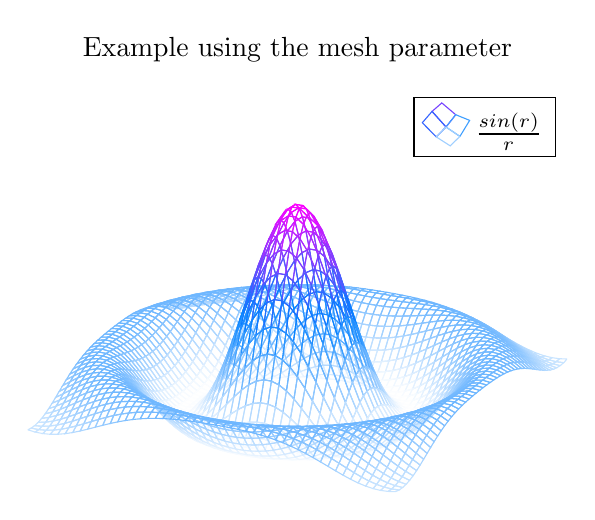
\begin{tikzpicture}
\begin{axis}[
    title=Example using the mesh parameter,
    hide axis,
    colormap/cool,
]
\addplot3[
    mesh,
    samples=50,
    domain=-8:8,
]
{sin(deg(sqrt(x^2+y^2)))/sqrt(x^2+y^2)};
\addlegendentry{\(\frac{sin(r)}{r}\)}
\end{axis}
\end{tikzpicture}


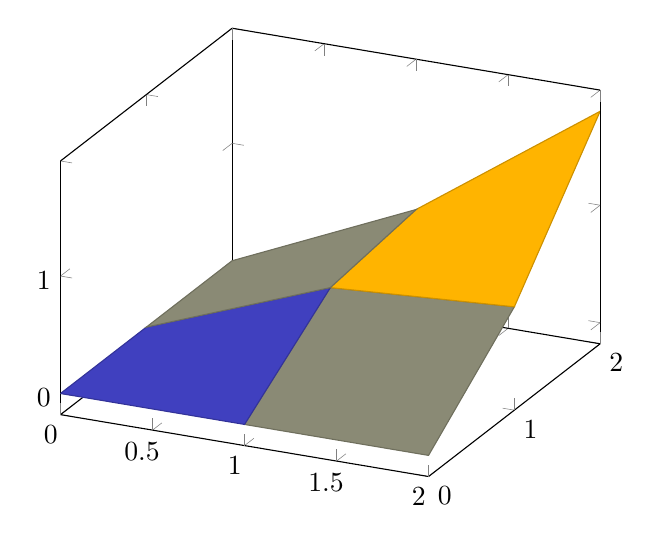
\begin{tikzpicture}
\begin{axis}
\addplot3[
    surf,
]
coordinates {
(0,0,0) (0,1,0) (0,2,0)

(1,0,0) (1,1,0.6) (1,2,0.7)

(2,0,0) (2,1,0.7) (2,2,1.8)
};
\end{axis}
\end{tikzpicture}

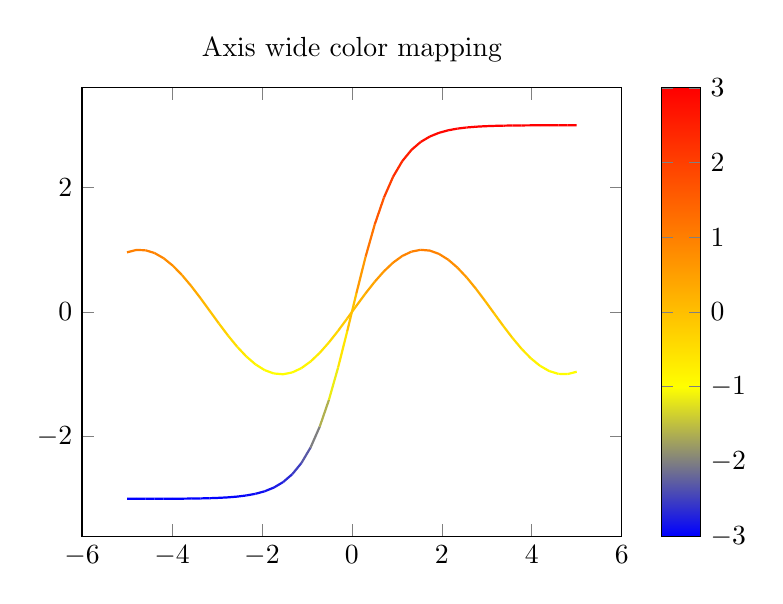
\begin{tikzpicture}
\begin{axis}[
title=Axis wide color mapping,
colorbar,
samples=50,point meta rel=axis wide,
point meta=y,
]
\addplot [mesh,thick] {sin(deg(x))};
\addplot [mesh,thick] {3*tanh(x)};
\end{axis}
\end{tikzpicture}


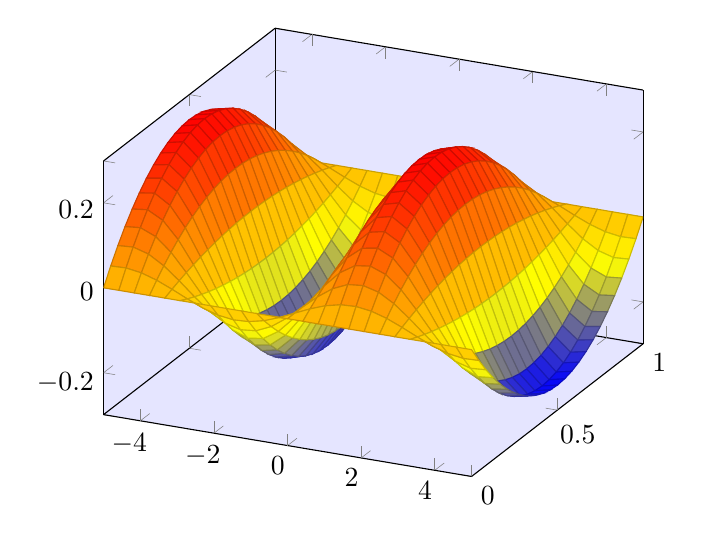
\begin{tikzpicture}
\begin{axis}[
axis background/.style={fill=blue!10},
]
\addplot3 [
surf,
y domain=0:1,
]
{sin(deg(x)) * y*(1-y)};
\end{axis}
\end{tikzpicture}

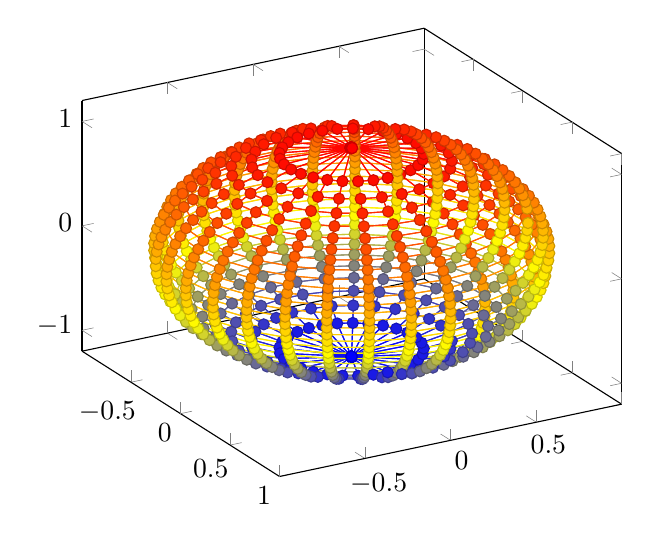
\begin{tikzpicture}
\begin{axis}[view={60}{30}]
\addplot3 [
only marks,
mesh,z buffer=sort,
scatter,scatter src=z,
samples=30,domain=-1:1,y domain=0:2*pi,
] (
{sqrt(1-x^2) * cos(deg(y))},
{sqrt( 1-x^2 ) * sin(deg(y))},
x
);
\end{axis}
\end{tikzpicture}




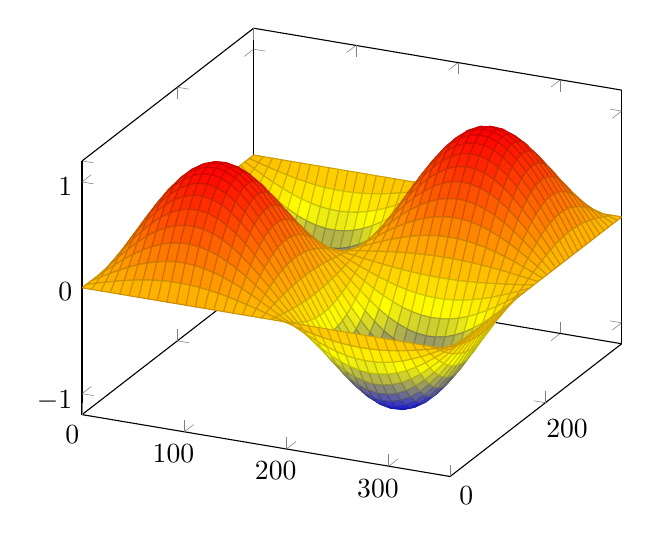
\begin{tikzpicture}
\begin{axis}
\addplot3 [
surf,
domain=0:360,
samples=40,
] {sin(x)*sin(y)};
\end{axis}
\end{tikzpicture}




\end{document}
